\newpage
\chapter{TINJAUAN PUSTAKA} \label{bab:tinjauan-pustaka}

\section{Tinjauan Pustaka} \label{sec:tinjauan-pustaka}
% Pembuka
Penelitian ini berangkat dari berbagai penelitian terdahulu yang membahas pengenalan bahasa isyarat (\textit{sign language recognition}) sebagai bagian dari pengenalan pola gerakan berbasis visual.
Penelitian-penelitian tersebut menunjukkan beragam pendekatan dalam memodelkan bahasa isyarat, baik dari sisi jenis bahasa isyarat yang dikenali maupun strategi pemodelan data gerakan.
Secara umum, pendekatan yang digunakan dapat diklasifikasikan berdasarkan cara memanfaatkan informasi temporal dan spasial dalam representasi data.
Tinjauan pustaka pada bagian ini disusun untuk mengkaji penelitian-penelitian yang relevan sebagai bahan perbandingan serta dasar dalam mengidentifikasi celah penelitian.
Uraian selanjutnya akan membahas beberapa penelitian terdahulu yang berkaitan dengan pengenalan bahasa isyarat, dimulai dari pendekatan berbasis temporal yang masih banyak digunakan hingga eksplorasi pendekatan berbasis spasial.

% Paper 1: Paper 1 (BISINDO + LSTM/GRU + MediaPipe)
% Real-Time BISINDO Sign Language Recognition: A Dynamic Approach with GRU and LSTM Models Leveraging MediaPipe (2023)
Penelitian oleh Yoses (2023) mengenai perbandingan LSTM dan GRU dalam klasifikasi BISINDO 

% Paper 2: Paper 6 (ResNet + LSTM)
% Video-Based Sign Language Recognition via ResNet and LSTM Network (2024)

% Paper 3: Paper 7 (Isolated SLR + Pose + ResNet–Transformer)
% Isolated Sign Language Recognition with Segmentation and Pose Estimation (2025)

% Paper 4: Paper 8 (Isolated SLR berbasis landmark MediaPipe dan kombinasi fitur)
% Multi-Stream Isolated Sign Language Recognition Based on Finger Features Derived from Pose Data (2024)

% Paper 5: Paper 2 (Fully 2D CNN untuk CSLR)
% Fully 2D Convolutional Network for Continuous Sign Language Recognition (2023)

Penelitian-penelitian yang menjadi referensi penulis dijabarkan pada Tabel \ref{table:2.literasi}. \par
% Tabel Ringkasan Penelitian

\renewcommand{\arraystretch}{1.0} % Mengatur spasi antar baris menjadi 1
\begin{longtable}{|c|p{0.22\textwidth}|p{0.22\textwidth}|p{0.21\textwidth}|p{0.16\textwidth}|}
  \caption{Literasi Penelitian Terdahulu}\label{table:2.literasi}\\
  \hline
  \textbf{No} 
    & \textbf{Penulis [Tahun] [Judul]} 
    & \textbf{Permasalahan} 
    & \textbf{Metode} 
    & \textbf{Hasil} \\ % ← you must end the row here
  \hline
\endfirsthead
  \hline
  \textbf{No} 
    & \textbf{Penulis [Tahun] [Judul]} 
    & \textbf{Permasalahan} 
    & \textbf{Metode} 
    & \textbf{Hasil} \\ % ← and here too
  \hline
\endhead
  \hline
\endfoot
  \hline
\endlastfoot
    1. 
    & Yoses Dwi Maheswara, M.Abid Al-Sulthon , Pradayan Adhimas Wicaksono, Khilda Afifah, dan Novi Prihatiningrum [2023] [\textit{Real-Time BISINDO Sign Language Recognition: A Dynamic Approach with GRU and LSTM Models Leveraging MediaPipe}] \cite{maheswara2023lstmbisindo}
    & Pendekatan statis kurang mampu menangkap dinamika gerakan BISINDO secara \textit{real-time}.
    & Ekstraksi \textit{landmarks} MediaPipe \textit{Holistic} dengan pemodelan temporal menggunakan LSTM dan GRU.
    & Model GRU mencapai performa terbaik dengan akurasi \textit{real-time} hingga 83\% pada kombinasi \textit{landmark} tanpa wajah. \\
    \hline
    2.
    & Jiayu Huang dan VarinChouvatut [2024][\textit{Video-Based Sign Language Recognition via ResNet and LSTM Network}] \cite{huang2024videoresnetlstm}
    & Ekstraksi fitur spasio-temporal video sulit dilakukan secara efisien dengan model CNN konvensional.
    & Arsitektur hibrida ResNet-18 sebagai ekstraktor spasial dan LSTM untuk pemodelan temporal.
    & Mencapai akurasi 86,25\% dan mengungguli beberapa model video-based lainnya. \\
    \hline
    3.
    & Daniel Perkins, Davis Hunter, Dhrumil Patel, dan Galen Flanagan [2025] [\textit{Isolated Sign Language Recognition with Segmentation and Pose Estimation}]
    & Model berbasis video sulit melakukan generalisasi akibat gangguan latar dan pencahayaan.
    & Integrasi estimasi pose, segmentasi, dan Bi-LSTM dengan Transformer berbasis pose.
    & Bi-LSTM dengan koordinat pose yang dinormalisasi mencapai performa tinggi sebesar 68,5\%.\\ 
    \hline
    4.
    & Ali Akdag dan Ömer Kaan Baykan [2024] [\textit{Multi-Stream Isolated Sign Language Recognition Based on Finger Features Derived from Pose Data}] 
    & Detail konfigurasi dan gerakan jari sering diabaikan dalam pengenalan bahasa isyarat.
    & Pendekatan multi-stream berbasis landmark jari dengan MobileNetV2, PCA, dan SVM.
    & Akurasi tinggi hingga 99,78\% pada dataset LSA64. \\
    \hline
    5.
    & Qidan Zhu, Jing Li, Fei Yuan dan Quan Gan [2023] [\textit{Fully 2D Convolutional Network for Continuous Sign Language Recognition}]
    & Model \textit{hybrid} spasio-temporal memiliki kompleksitas tinggi dan ketergantungan arsitektur sekuensial.
    & F2DCNet berbasis 2D CNN murni dengan penggabungan fitur temporal dalam representasi input.
    & Mencapai \textit{Word Error Rate} (WER) terendah hingga 20,0\% pada dataset skala besar.\\ 
\end{longtable}

% Analisis Celah Penelitian

\section{Dasar Teori} \label{sec:dasar-teori}
Berikut ini merupakan dasar teori yang digunakan pada penelitian ini: \par

\subsection{Bahasa Isyarat Indonesia (BISINDO)} \label{subsec:bisindo}
Denyut yang dirasakan sebenarnya bukan darah yang dipompa langsung oleh jantung ke aorta, melainkan gelombang tekanan yang berasal dari aorta yang merambat lebih cepat dibandingkan aliran darah itu sendiri. \par

\subsection{\textit{Isolated Sign Language Recognition}} \label{subsec:islr}


\lipsum[1-2] % Menampilkan paragraf 1 sampai 2 dari lorem ipsum
Gambar yang digunakan \ref{fig:3.ref_gbr}. \par
\begin{figure}[H] % Kalau menggunakan H, posisi gambar akan tepat dibawah teks
    \centering
    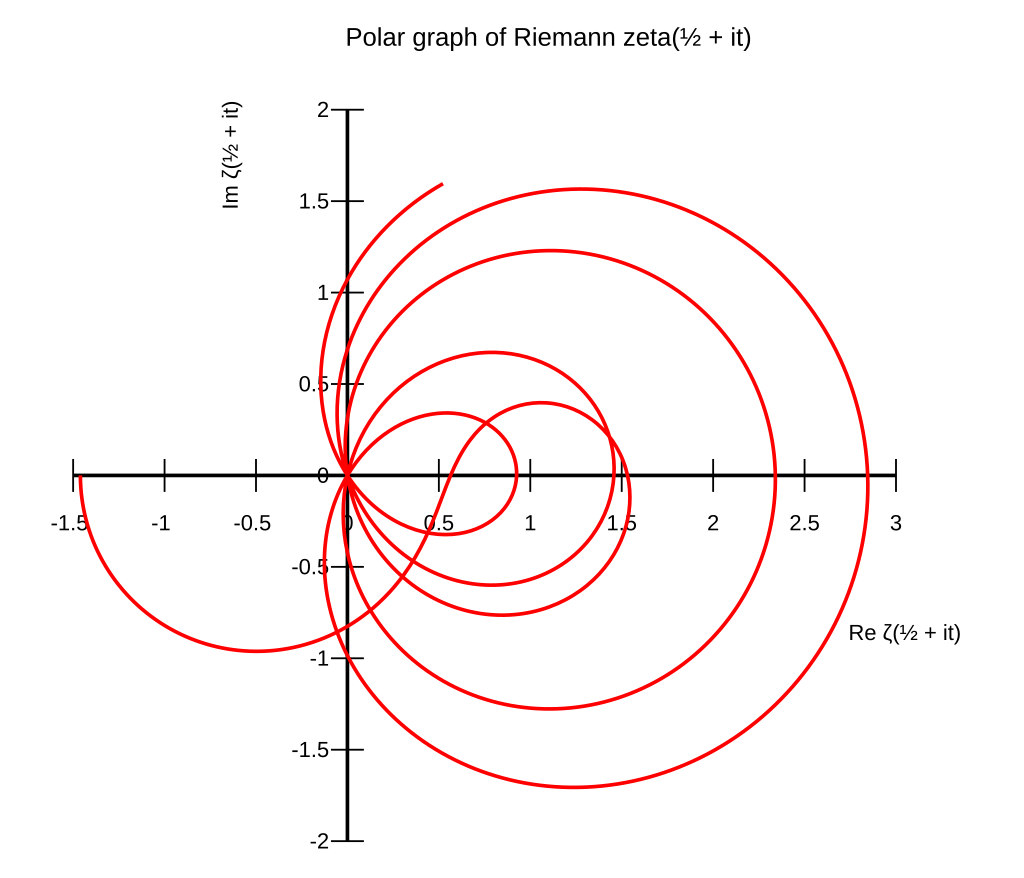
\includegraphics[width=0.6\textwidth]{figure/zeta.png}
    \caption{Referensi Gambar}
    \label{fig:3.ref_gbr}
    {\footnotesize Sumber: internet}
\end{figure}

\subsection{Representasi Landmark Tubuh Manusia} \label{subsec:landmark}

Berikut adalah ilustrasi konsep yang digunakan seperti pada Gambar \ref{fig:3.ref_gbr2}. \par
\begin{figure}[H] % Posisi gambar tepat dibawah teks
  \centering
  
\includegraphics[width=0.7\textwidth]{figure/Logo_ITERA.png}
  \caption{Ilustrasi Konsep}
  \label{fig:3.ref_gbr2}
  {\footnotesize Sumber: dokumentasi penelitian}
\end{figure}

\subsection{\textit{Mediapipe Holistic}} \label{subsec:mediapipe}
\textit{Mean Absolute Error} (MAE). Rumus perhitungan dari MAE dapat dilihat pada \ref{eq:2.mae}. \par

\begin{equationcaptioned}[eq:2.mae]{
    MAE = \frac{1}{n} \sum_{i=1}^{n} \left| y_i - \hat{y}_i \right|
}{
    Mean Absolute Error (MAE)
}
\end{equationcaptioned}

\subsection{Representasi Spasial Landmark Multichannel} \label{subsec:multichannel}
\subsection{\textit{Convolutional Neural Network} (CNN) 2D} \label{subsec:cnn2d}
\subsection{\textit{Residual Network} (ResNet)} \label{subsec:resnet}
\subsection{Modifikasi Input Channel pada CNN} \label{subsec:modifikasi-cnn}
\subsubsection{CNN tidak terbatas pada input RGB}
\subsubsection{Penerimaan arbitrary number of channels}
\subsubsection{Contoh Penerapan Non-RGB}
\subsection{Metrik Evaluasi Klasifikasi} \label{subsec:metrik-evaluasi}
